%!TEX program = pdflatex
\documentclass[conference]{IEEEtran}


  \usepackage{ifluatex}

  \ifluatex
    \usepackage{fontspec}
    %\defaultfontfeatures{Ligatures=TeX} 
    % load your system fonts; e.g.:
    %\setmainfont{LinLibertineO}
    %\setsansfont{LinBiolinumO}
    %\setmonofont{Inconsolata}
  \else
    \usepackage[utf8]{inputenc}                   
    \usepackage[T1]{fontenc}
    % load some Type 1 font; e.g.:
    %\usepackage[fulloldstylenums,largesmallcaps]{kpfonts}
  \fi

  \usepackage{units}

  \usepackage{glossaries}

  \usepackage{subcaption} % will be problematic for llncs
  \captionsetup{compatibility=false} 

  \usepackage{xspace}

  \usepackage{tikz}
\usetikzlibrary{arrows}

\usepackage{booktabs}

\usepackage{url}
\usepackage{mathtools}
\usepackage{fixmath}

\usepackage{tabu}

\setlength{\belowcaptionskip}{-5pt}

\definecolor{grey}{RGB}{153, 153, 153}
\definecolor{orange}{RGB}{230, 159, 0}
\definecolor{skyblue}{RGB}{86, 180, 233}
\definecolor{bluishgreen}{RGB}{0, 158, 115}
\definecolor{yellow}{RGB}{240, 228, 66}
\definecolor{blue}{RGB}{0, 114, 178}
\definecolor{vermillion}{RGB}{213, 94, 0}
\definecolor{reddishpurple}{RGB}{204, 121, 167}

\newcommand{\blockingprobability}[0]{p_B}
\newcommand{\maxServers}[0]{S_{\max}}

%!TEX root = paper.tex
\newacronym{3GPP}{3GPP}{Third Generation Partnership Project}
\newacronym{DoS}{DoS}{Denial of Service}
\newacronym{GGSN}{GGSN}{Gateway GPRS Support Node}
\newacronym{GPRS}{GPRS}{General Packet Radio Service}
\newacronym{GSM}{GSM}{Global System for Mobile Communications}
\newacronym{GTP}{GTP}{GPRS Tunneling Protocol}
\newacronym{IE}{IE}{Information Element}
\newacronym{IMEI}{IMEI}{International Mobile Equipment Identity}
\newacronym{IMSI}{IMSI}{International Mobile Subscriber Identity}
\newacronym{METAWIN}{METAWIN}{Measurement and Traffic Analysis in Wireless Networks}
\newacronym{MS}{MS}{Mobile Station}
\newacronym{MS-ID}{MS-ID}{Mobile Station Identifier}
\newacronym{PDP}{PDP}{Packet Data Protocol}
\newacronym{QoS}{QoS}{Quality of Service}
\newacronym{RAB}{RAB}{Radio Access Bearer}
\newacronym{RAT}{RAT}{Radio Access Technology}
\newacronym{RNC}{RNC}{Radio Network Controller}
\newacronym{RRC}{RRC}{Radio Resource Control}
\newacronym{SGSN}{SGSN}{Serving GPRS Support Node}
\newacronym{TAC}{TAC}{Type Allocation Code}
\newacronym{TS}{TS}{Technical Specification}
\newacronym{UMTS}{UMTS}{Universal Mobile Telecommunications System}
\newacronym{UTRAN}{UTRAN}{UMTS Terrestrial Radio Access Network}
\newacronym{DES}{DES}{Discrete Event Simulation}
\newacronym{CDF}{CDF}{Culmulative Distribution Function}
\newacronym{SSD}{SSD}{Solid State Disk}
\newacronym{NFV}{NFV}{Network Function Virtualization}
\newacronym{SDN}{SDN}{Software Defined Networking}


\makeglossaries


\usepackage[url=true,doi=false,backend=biber,style=ieee,sorting=none,minnames=1,maxnames=2]{biblatex}
\addbibresource{literature.bib}

\newcommand{\refsec}[1]{Sec.~\ref{sec:#1}}
\newcommand{\reffig}[1]{Fig.~\ref{fig:#1}}
\newcommand{\reftab}[1]{Tab.~\ref{tab:#1}}



\begin{document}

\title{GTP-based Load Model and Virtualization Gain for a Mobile Network's GGSN}

\author{\IEEEauthorblockN{Florian Metzger}
\IEEEauthorblockA{University of Vienna, Austria\\
Future Communication Research Group\\
florian.metzger@univie.ac.at}
\and
\IEEEauthorblockN{Christian Schwartz and Tobias Hoßfeld}
\IEEEauthorblockA{University of Würzburg, Germany \\
Chair of Communication Networks\\
{christian.schwartz,tobias.hossfeld}@informatik.uni-wuerzburg.de}}

\maketitle

%!TEX root = paper.tex
\begin{abstract}
Multiple outages in major mobile networks have been reported in the recent past. In fixed and datacenter networks such capacity problems are solved by scaling out, i.e. purchasing additional hardware. In mobile networks this is not as easily possible as network components are usually sold as sealed middleboxes. With the advances in server performance and SDN it has been suggested to virtualize these boxes. This also opens up opportunities to dimension according to current load and save energy by switching off parts of the infrastructure.

Such suggestions immediately raise questions on the cost of virtualization. To answer this, we introduce models for both a traditional as well as a virtualized GGSN. In addition, we provide distributions for the load experienced at the GGSN based on network measurements. With this at hand, we study the influence of different dimensioning parameters on important performance metrics, with special consideration for the impact of provisioning new instances for the virtual GGSN.
\end{abstract}

%!TEX root = paper.tex
\section{Introduction}
\label{sec:intro}
With the increased importance of smart phones, mobile networks are currently experiencing rapid growth.
Compared to a fixed access provider additional aspects have to be taken into account when dimensioning a mobile network. 
First and most prominent is the planning of radio access cells --- their coverage, frequency selection, and backhaul, i.e., the connection to the operator's network. Radio network planning research and tools readily exist to help solve this problem \cite{tutschku1998demand}.
Albeit of equal importance, there is much less public knowledge and research on the second aspect in setting up the mobile network: setting up and dimensioning the core network. Consisting of a large number of specialized network nodes in need of careful tuning to each other, correctly putting together the core is no small feat. The reason for this is the large number of services incorporated into the protocol stack --- e.g., authentication, accounting, or monitoring --- and the amount of state, that needs to be held and signaled throughout the network, coming with it.

One major metric to consider in this core dimensioning is the number of supported tunnels, i.e., connections to the Internet, of the \gls{GGSN}.
The \gls{GGSN}'s performance depends on factors like customers to serve, applications in the network, user behavior and devices used. During dimensioning, these factors are either unknown or subject to change as user behavior evolves.
But these network components are sold as static middleboxes and cannot not be easily extended with of-the-shelf hardware in order to account for new requirements.
The newly introduced concept of \gls{NFV}~\cite{nfv_whitepaper} suggests to harness technologies from cloud computing in the network. This would allow network operators to scale out, i.e., using additional low performance machines, instead of scaling up, which requires them to replace existing hardware with more powerful components.

The contribution of this work is threefold. First, we introduce models for both a traditional \gls{GGSN} as well as a virtual \gls{GGSN} using \gls{NFV}. Second, we provide distributions for \gls{GTP} tunnel interarrival times and durations. Finally, we study performance trade-offs when using a virtual \gls{GGSN}, discussing different options to consider when using a virtual \gls{GGSN}.

This paper is structured as follows. Section~\ref{sec:background} gives a brief explanation of the involved 3G infrastructure and general behavior of mobile networks. An overview of the related work is also included. We present our two models in Section~\ref{sec:model}. Afterwards, Section~\ref{sec:dataset} consists of a short description of the dataset that was used and the relevant evaluations and conclusions drawn from the data. Afterwards, we evaluate the numerical results and implications of the queuing simulation in Section~\ref{sec:numerical}. The paper concludes in Section~\ref{sec:conclusion}.

%!TEX root = paper.tex
\section{Background}
\label{sec:background}
This section provides the necessary background on topics important for the remainder of the paper including \gls{GPRS} basics and related work.
%\gls{GPRS}, and therefore \gls{UMTS} fundamentals, and \gls{GTP} signaling are discussed in \refsec{gprs_fundamentals}.
%A short overview of related work is given in \refsec{related_work}.
\subsection{\acrshort{GPRS} \& \acrshort{UMTS} Fundamentals}\label{sec:gprs_fundamentals}
UMTS is specified by the \gls{3GPP}, with relevant parts for this investigation found in \gls{TS} 23.060~\cite{3gpp23060}, which defines the network's basic aspects involving \gls{GPRS} protocols and its system architecture, and \gls{TS} 29.060~\cite{3gpp29060}, describing the specifics of \gls{GTP} across the Gn and Gp interfaces.

The \gls{SGSN} and the \gls{GGSN} are the main components in the core's packet switched domain.
The \gls{SGSN} serves mainly as mobility anchor, the \gls{GGSN} represents the gateway to the public Internet and is responsible for most connection and transmission related management. All user traffic between these nodes is encapsulated in a tunnel and managed with explicit \gls{GTP} signaling.

Tunnel state is kept in the \gls{SGSN} and \gls{GGSN} as \gls{PDP} Context data structures.
These contain various information, such as the device's IP address, \gls{IMSI}, and a tunnel identifier.
Usually, any user-plane IP traffic is transported within a primary ``best effort'' tunnel.
The \gls{GTP} signaling, responsible for the context management interactions, contains procedures for managing data paths, \gls{MS} locations, mobility, and, of course, tunnels.
Of relevancy to this paper are the tunnel management request/response message pairs involved in the maintenance of \gls{PDP} Contexts.

\subsection{Related Work}
\label{sec:related_work}

This work is a continuation of our previous evaluations conducted in \cite{metzger2012research, metzger2014jcnc}.
Besides these, there is to our knowledge no other directly preceding literature to this paper's novel models.
Still, efforts have been made to investigate the special properties of mobile networks and its traffic.
These include attempts to infer control plane behavior through active measurements at the mobile device or synthetic traces and investigations of user traffic characteristics by means of real 3G core network traces.
The authors of \cite{qian2011profiling} discuss cross-layer interactions in mobile cellular networks and the consequences for device energy consumption and radio channel allocation efficiency.

Looking at the multitude of radio network control state machines, we find in \cite{5360763} some simple yet effective application layer methods investigating transitions of these state machines.This is further elaborated on by \cite{schwartz2013angrybirds} in order to analyze the radio signaling load and thus power efficiency from several different applications.

Having access to core network datasets, the authors of \cite{shafiq2011characterizing, paul2011understanding} both take the approach of looking at high-level user traffic characteristics, focusing on temporal and spatial variations of user traffic volume and investigating the influence of different devices on this metric.
Additional user flow and session traffic metrics are being studied in \cite{Zhang:2012:UCC:2377677.2377764} with the conclusion that, in comparison to wired traffic, short flows are occurring more frequently.
In 2006, a core network measurement study of various user traffic related patterns was conducted, providing an initial insight into \gls{PDP} context activity and durations \cite{svoboda2006composition}.


%In \cite{lee2007detection}, mobile network traces are used to simulate a malicious signaling storm by transmitting low-volume user plane traffic with specially crafted inter-departure times, causing signaling to occur constantly.
%The authors of \cite{4675847} give some thoughts on the influence of core network elements on one-way delays in mobile networks.
%!TEX root = paper.tex
\section{Model}
\label{sec:model}
In this section we provide a model for a traditional \gls{GGSN} and discuss a model for a virtual \gls{GGSN} using \gls{NFV}. In \gls{NFV}~\cite{nfv_whitepaper} static network middleboxes are replaced by commodity hardware. The tasks solved by the original middleboxes are then handled by dedicated software. The generic queuing theoretic model is based on observations drawn from the measurement set provided in \refsec{dataset}. As such, any properties outside these observations are not reflected.

\begin{figure}[htbp]
  \centering
  \resizebox{0.8\columnwidth}{!}{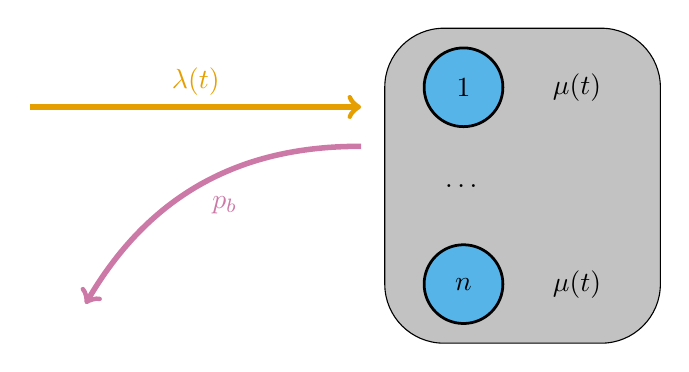
\begin{tikzpicture}
  [
    flow/.style={line width=2pt, =>stealth'},
    arrival/.style={flow, orange},
    block/.style={flow, reddishpurple},
    ggsn/.style={fill=grey!60, rounded corners=0.75cm},
    server/.style={line width=1pt, fill=skyblue}
  ]
  \draw[->, arrival] (0.0, 3.0)  -- node[above] {$\lambda(t)$} (4.2, 3.0);
  \draw[block, bend right] (4.2, 2.5) edge[->] node[below right] {$p_b$} (0.7, 0.5);

  \draw[ggsn] (4.5, 0.0) rectangle (8.0, 4);

  \draw[server] (5.5, 3.25) circle[radius=0.5cm] node {$1$} node[right=1.0cm] {$\mu(t)$};
  \draw (5.5, 2.00) node {\textellipsis};
  \draw[server] (5.5, 0.75) circle[radius=0.5cm] node {$n$} node[right=1.0cm] {$\mu(t)$};
\end{tikzpicture}

}
  \caption{Model of a Traditional GGSN}
\label{fig:model_traditional_ggsn}
\end{figure}

While internally a \emph{traditional} \gls{GGSN} may consist of multiple individual servers, it acts as a monolithic entity from an outside point of view. Therefore, idle portions of it can neither be deactivated nor reused for other purposes. This first model is based on this monolithic idea.

The queuing theory equivalent to this model is displayed in Figure~\ref{fig:model_traditional_ggsn}. New tunnels requests arrive according to a Poisson distribution with a rate of $\lambda(t)$ at the GGSN, which has a maximum tunnel capacity of $c_c$. When the capacity is reached, blocking will occur and newly incoming tunnels are rejected. Traditionally, \glspl{GGSN} can be expected to be overdimensioned in such a way, that this rarely happens. If an incoming tunnel request is accepted, one of the \gls{GGSN}'s serving units will be occupied for the tunnel's duration of $\mu(t)$. The duration is assumed to be of an arbitrary non-Markovian service time distribution. Together this results in a non-stationary Erlang loss model, or $M(t)/G/c_c/0$.

In order to give QoS guarantees the network operator is interested in the system's blocking probability $\blockingprobability$, which we consider to be a key metric of our model.
Additionally, the previously described diurnal patterns can also be modeled by adjusting the arrival and serving process distributions for each time of day. This alternatively also allows just to investigate the busy hour and thus the system's peak load.

\subsection{GGSN using Network Function Virtualization}\label{sec:virtual_ggsn}
\begin{figure}[htbp]
  \centering
  \resizebox{0.9\columnwidth}{!}{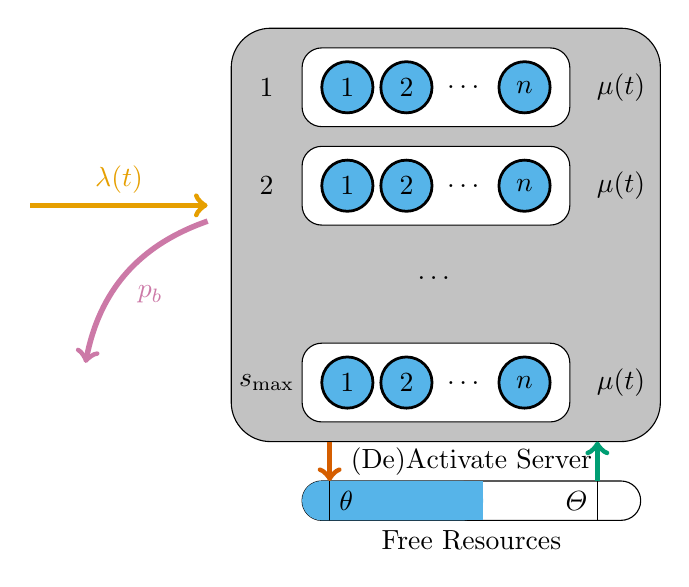
\begin{tikzpicture}
  [
    flow/.style={line width=2pt, =>stealth'},
    arrival/.style={flow, orange},
    block/.style={flow, reddishpurple},
    ggsn/.style={fill=grey!60, rounded corners=0.5cm},
    server/.style={line width=1pt, fill=skyblue},
    vm/.style={fill=white, rounded corners=0.25cm},
    resources/.style={rounded corners=0.25cm},
    activate/.style={->, bluishgreen, line width=2pt},
    deactivate/.style={<-, vermillion, line width=2pt}
  ]
  \draw[->, arrival] (0.0, 3.0)  -- node[above] {$\lambda(t)$} (2.25, 3.0);
  \draw[block, bend right] (2.25, 2.8) edge[->] node[below right] {$p_b$} (0.7, 1.0);

  \draw[ggsn] (2.55, 0.0) rectangle (8.0, 5.25);

  \draw[server] (3.0, 0.75) node {$s_{\max}$};

  \draw[vm] (3.45, 0.25) rectangle (6.85, 1.25);
  \draw[server] (4.025, 0.75) circle[radius=0.325cm] node {$1$};
  \draw[server] (4.775, 0.75) circle[radius=0.325cm] node {$2$};
  \draw[server] (5.525, 0.75) node {\textellipsis};
  \draw[server] (6.275, 0.75) circle[radius=0.325cm] node {$n$};
  \draw[server] (7.500, 0.75) node {$\mu(t)$};

  \draw (5.15, 2.075) node {\textellipsis};

  \draw[server] (3.0, 3.25) node {$2$};

  \draw[vm] (3.45, 2.75) rectangle (6.85, 3.75);
  \draw[server] (4.025, 3.25) circle[radius=0.325cm] node {$1$};
  \draw[server] (4.775, 3.25) circle[radius=0.325cm] node {$2$};
  \draw[server] (5.525, 3.25) node {\textellipsis};
  \draw[server] (6.275, 3.25) circle[radius=0.325cm] node {$n$};
  \draw[server] (7.500, 3.25) node {$\mu(t)$};

  \draw[server] (3.0, 4.5) node {$1$};

  \draw[vm] (3.45, 4) rectangle (6.85, 5);
  \draw[server] (4.025, 4.5) circle[radius=0.325cm] node {$1$};
  \draw[server] (4.775, 4.5) circle[radius=0.325cm] node {$2$};
  \draw[server] (5.525, 4.5) node {\textellipsis};
  \draw[server] (6.275, 4.5) circle[radius=0.325cm] node {$n$};
  \draw[server] (7.500, 4.5) node {$\mu(t)$};

  \draw (5.6, -0.25) node {(De)Activate Server};
  \draw[resources] (3.45, -1.0) rectangle(7.75, -0.5);
  \fill[skyblue, resources] (3.45, -1.0) rectangle(5.75, -0.5);
  \fill[skyblue] (3.8, -1.0) rectangle(5.75, -0.5);
  \draw (3.8, -1.0) rectangle node[right] {$\theta$} (3.8, -0.5);
  \draw[deactivate] (3.8, -0.5) -- (3.8, 0.0);
  \draw (7.2, -1.0) rectangle node[left] {$\Theta$} (7.2, -0.5);
  \draw[activate] (7.2, -0.5) -- (7.2, 0.0);
  \draw (5.6, -1.25) node {Free Resources};

\end{tikzpicture}

}
  \caption{Model of a GGSN using Network Function Virtualization}
  \label{fig:model_nfv_ggsn}
\end{figure}

In the second model, we introduce concepts from \gls{NFV}, i.e., the idea to replace middleboxes with commodity hardware.
This allows us to realize benefits from cloud computing, as we are now able to scale out instead of up. The assumptions of the Markov arrival process $\lambda(t)$ and the serving time distributions $\mu(t)$ are carried over. However, instead of one server processing every tunnel, this model assumes that there are up to $s_{max}$ virtualized servers $s_i$. Each of these can be much smaller than the traditional GGSN, having a tunnel serving capacity of $c_i \ll c_c$ and a total system capacity of $c_{max} = s_{max} \times c_i$.

To increase efficiency all but a small portion of the server instances can be initially turned off. Only when a certain condition is reached, a new one needs to be provisioned. For example, one could always hold one instance in reserve for upcoming requests and provision as soon as the reserver gets used. Similar rules should apply in the shutdown of servers and should form a hysteresis together with the boot condition. 
%For example it would be possible to keep at least one server in reserve but never more than two.

If these conditions are not carefully selected and are in tune with the expected boot time of an instance, additional blocking could occur. Despite not having reached its maximum capacity, this system will still reject tunnel requests during the provisioning phase when no tunnel slots are free. This could be remedied by a request queue. However, this makes the system more complex without providing real benefit, as mobile devices usually just repeat their attempts when the request is taking too long. 

To place incoming tunnel state on one of the available servers and manage the servers a load balancer or hypervisor is required. To ensure, that the system can scale down to its actual needs, the balancer should place tunnels on servers, that are the fullest, keeping the reserve free. It may even migrate tunnel state from almost empty servers away so that these can be shut down, when certain conditions are fulfilled. Keeping instance close to their capacity should also have no impact on the performance a mobile device associated to a specific tunnel experiences. Adequate strategies for both load balancing and migration will be considered in future work.

%!TEX root = paper.tex
\section{The Data}
\label{sec:dataset}
In order to evaluate the newly introduced models we use data collected from a nation-wide mobile operator. This allows for precise core network evaluations and the creation of statistical fits for the observed processes.
In this section we first describe the dataset used for the evaluation and afterwards we derive the random variables required for our models.

\subsection{Dataset Description}
\label{sec:dataset_description}
All data was collected by the \gls{METAWIN} monitoring system~\cite{ricciato_2011} with measurement probes located at the Gn interface within the core network, enabling broad access to signaling. For this investigation we exclusively use \gls{GTP} protocol data which was fully anonymized to meet privacy requirements.

The dataset used in our evaluation is a week-long trace from the third week of April 2011. It contains $410$ million \gls{GTP} tunnel management transactions, and was tapped at one of the operator's \gls{GGSN} locations, handling about half of the operator's total traffic volume in this period.
%The records were stored in a SQL database, with most of the statistical evaluation conducted using R.

\subsection{Statistical Evaluation}\label{sec:statistical_evaluation}
\begin{figure}[htbp]
  \centering
  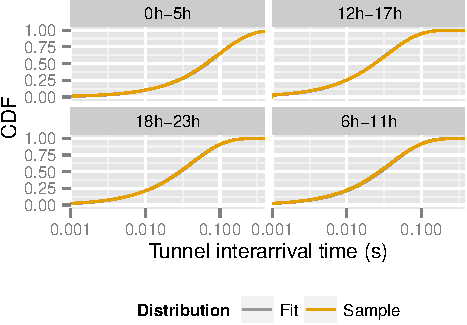
\includegraphics[width=1.0\columnwidth]{figures/R-IAT-active-fit-cdf-facets.pdf}
  \caption{Empirical and exponentially fitted CDFs of the tunnel interarrival duration by time of day. CDFs are overlapping as the coefficient of determination is close to $1$.}
  \label{fig:pdparrivalsecdf}
\end{figure}
Using this dataset, we can now compare the processes in our proposed models with the empirical distributions from actual data. First, we take a look at the tunnel interarrival time in Figure~\ref{fig:pdparrivalsecdf}.
%Tunnels can be initiated and shut down in rapid succession, thus causing the aforementioned issues in the radio network.
The arrivals show a strong diurnal effect, closely resembling patterns also present in user plane traffic.
In the data we see a decline of arrivals, i.e., longer interarrivals, late in the night and during the early morning hours with a peak rate in the afternoon and early evening.
To represent this time-of-day dependence in the model, the measurement was split into the four time slots displayed in the figure.
Each slot was then fitted with an exponential distribution with the rates $\lambda$ given in Table~\ref{tab:fits} for the four time slots.
The fitted functions match the empirical data, with some deviation present at the left tail but overall with a correlation coefficient approaching positive $1$.
\begin{figure}[htbp]
  \centering
  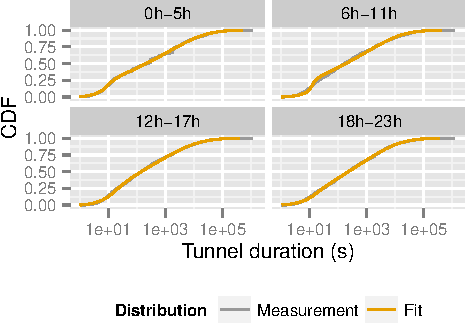
\includegraphics[width=1.0\columnwidth]{figures/timeslot-fits.pdf}
  \caption{Empirical and fitted CDFs of the tunnel duration by time of day with fitted rational functions.}
  \label{fig:fittedsdurationlots}
\end{figure}
Next, we consider the duration the \gls{PDP} Context state, which accompanies any \gls{GTP} tunnel, is held at the \gls{GGSN}.
Fig.~\ref{fig:fittedsdurationlots} shows the tunnel durations split up for the time of day. There is once again a slight diurnal effect present, albeit with shifted peaks. Longer tunnels tend to occur at night, shorter tunnels during midday.
For the model a distribution fit of the tunnel duration was also desired.
However, none of the basic probability distributions (including exponential, gamma, and Weibull distributions) fit the tunnel duration well enough.
We assume, that this can be attributed to the correlation of the tunnel duration to a large number of external factors, including user behavior, network-specific timers and procedures. All of which introduce artifacts and make it difficult to fit any distribution against.
To get some kind of approximate mathematical representation of this distribution regardless, we attempted a rational function fit using Eureqa \cite{eureqa_paper}.
%, allowing for a much closer fitting while still smoothing out some of the artifacts.
Table~\ref{tab:fits} additionally displays the generated functions which were fitted to the inverse CDF\footnote{The inverse CDF was chosen as target to be able to directly use them in the random number generator in our simulation.}. 
Both the CDFs in Fig.~\ref{fig:fittedsdurationlots} as well as the Pearson correlation coefficients confirm the goodness of the fitted functions.
\begin{table}[htbp]
  \caption{Parameters for the exponentially distributed inter-arrival times and corresponding Pearson correlation coefficients as well as the inverse functions fitted to the empirical duration distribution and correlation coefficients of the fit.}
  \label{tab:fits}
  \tabcolsep=0.11cm
  \centering
  \begin{tabu}{X[2,l]X[r]X[r]X[4.5,r]X[r]} 
  \toprule
  Time of Day & $\lambda$ & $R_{arr}$ & Inverse Fitted Duration Function & $R_{dur}$\\% \tabucline[1pt]-\everyrow{\tabucline[on 1.5pt off 2pt] -
  \midrule
  0h-5h & $10.67$ & $0.99$ & $0.91 - 60.61y - 3498.78y^3 - \frac{110.70y + 2289.94y^3}{y - 1.00}$ &  $0.99$ \\
  6h-11h & $24.53$ & $0.99$ & $1 + 117.48y - 368.64y^2 - \frac{1720.13y^4}{y - 1.00}$ & $0.99$ \\
  12h-17h & $29.25$ & $0.99$ & $0.95 + 69.49y + \frac{81146.10y^3 + 1.08\times10^6y^5}{805 - 802.01y}$ & $0.99$ \\
  18h-23h & $23.49$ & $0.98$ & $0.91 + 82.05y - \frac{2936.93y^4}{1.94y - 1.95}$ & $0.99$ \everyrow{} \\ \bottomrule
  \end{tabu}
\end{table}

%!TEX root = paper.tex
\section{Numerical Evaluation}
\label{sec:numerical}
We implement\footnote{\url{https://github.com/fmetzger/ggsn-simulation/}} the models introduced in \refsec{model} using a \gls{DES} with the SimPy \cite{simpy} package as foundation.
To be in line with the measurement data we consider a simulation time of seven days for all simulation scenarios, with a transient phase of 60 minutes accounted for. Ten replications of each scenario were performed.
All error bars given in this section show the $5\%$ and $95\%$ quantiles of all replications.

In \refsec{eval_traditional_ggsn} we use the measurements introduced in \refsec{dataset} in order to dimension a traditional \gls{GGSN} as a baseline for all further studies.
Based on these results, in \refsec{virtual_ggsn} we examine the effects of \gls{NFV} by scaling \emph{out} instead of up in \refsec{eval_ideal_virtual_ggsn} through a virtual \gls{GGSN} model. Finally, we arrive at a more realistic version of the virtual \gls{GGSN} by taking the start up and shut down times into account in \refsec{real_virtual_ggsn}.

\subsection{Traditional GGSN}
\label{sec:eval_traditional_ggsn}
With the help of the interarrival times and duration of tunnels we study the traditional \gls{GGSN} model previously introduced.
Whilst our measurements provided us with information on the frequency of new tunnels and the duration they remain active, we have no reliable information on the number of active tunnels the \gls{GGSN} can support. Thus, in a first step, we dimension the \gls{GGSN} in such a way that a suitable blocking probability $\blockingprobability$ can be achieved.

To obtain a baseline dimensioning, we perform a simulation study that considers the impact of an increasing load offer on the blocking probability.
We find that for the normalized interarrival time no blocking is occurring if we allow for more than $5000$ parallel tunnels.
Thus, we consider the range of $4000$ to $5000$ parallel tunnels to be of special interest for the remainder of the study.

\subsection{Virtual \gls{GGSN}}
\label{sec:eval_ideal_virtual_ggsn}
In order to study the feasibility of the virtual \gls{GGSN} approach discussed in \refsec{virtual_ggsn}, we compare the performance indicators of the virtual \gls{GGSN} with that of a traditional \gls{GGSN}.
To this end, the virtual \gls{GGSN} is simulated in varying configurations.
The number of servers and supported tunnels per server is chosen in such a way that the results can be compared with those obtained from our study of the traditional \gls{GGSN}.

In the virtual \gls{GGSN} model, servers are activated and deactivated on demand, while in the traditional \gls{GGSN} model, the single server is always on.
%For this investigation a conservative start up and shut down time of \unit[300]{seconds} is chosen.
Generally, deactivating server instances reduces energy consumption and frees up inactive servers for other use.
Thus, the number of active servers is a relevant performance metric.
%!TEX root = paper.tex
\begin{table}\caption{Manipulation check for the experimental factors based on one-way ANOVA.}
\centering
\label{tab:manipulation2color}
\tabcolsep=0.11cm
\begin{tabu}{lrrrcc}
\toprule
& \multicolumn{1}{c}{$F(2,1275)$} & \multicolumn{1}{c}{$\eta^2_p$} & \multicolumn{1}{c}{$p$} & Cohen's & Cohen's\\ 
&  & & & $f^2$ & $\hat{\omega}^2$ \\ 
\midrule
\emph{blocking probability}  & & & & &\\ 
maxTunnels &  $15601.53$ & $\textcolor{red}{0.993}$ & $<0.001$ & $\textcolor{red}{26.73}$ & $0.96$\\ 
maxInstances &  $10218.17$ & $\textcolor{red}{0.986}$ & $<0.001$ & $\textcolor{red}{1.06}$ & $0.51$\\ 
startstopDuration &  $0.86$ & $\textcolor{black}{0.003}$ & $0.482$ & $\textcolor{black}{0.00}$ & $0.00$\\ 
\midrule
\emph{mean tunnel count}  & & & & &\\ 
maxTunnels &  $20448.34$ & $\textcolor{red}{0.994}$ & $<0.001$ & $\textcolor{red}{27.71}$ & $0.96$\\ 
maxInstances &  $13348.25$ & $\textcolor{red}{0.989}$ & $<0.001$ & $\textcolor{red}{1.06}$ & $0.51$\\ 
startstopDuration &  $2.87$ & $\textcolor{black}{0.009}$ & $0.022$ & $\textcolor{black}{0.00}$ & $0.00$\\ 
\bottomrule
\end{tabu}
\end{table}
 % with \label{tab:manipulation2color}
In order to analyze the influence of the different model parameters on the performance metrics, we perform a one-way ANOVA analysis with the results collected in \reftab{manipulation2color}.
High values for $\eta_p^2$ and Cohen's $f^2$~\cite{stats} indicate that the main influence for both the blocking probability and mean number of tunnels is the maximum number of tunnels $n$ and servers $\maxServers$, i.e., the total number of possible concurrent tunnels in the system.
\begin{figure}[htbp]
  \begin{center}
  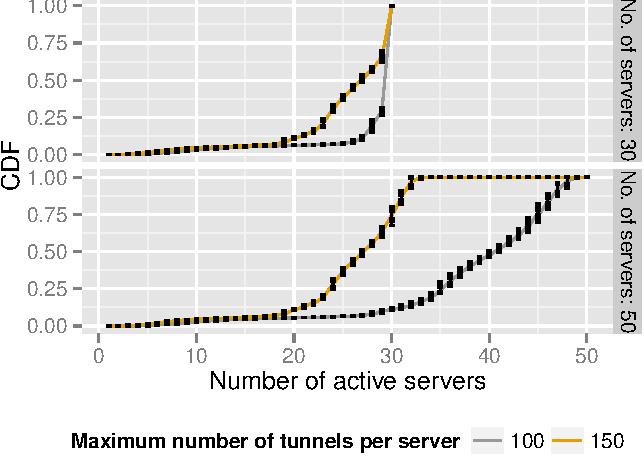
\includegraphics[width=1.0\columnwidth]{figures/instanceuse-multiserver-real.pdf}
  \caption{Impact of the maximum number of tunnels and servers on number of active servers in the virtual \gls{GGSN} model.}
\label{fig:instance_use_virtual}
  \end{center}
\end{figure}
In \reffig{instance_use_virtual} the \gls{CDF} of the number of active servers for four different virtual \gls{GGSN} configurations is displayed.
We observe, that increasing the number of supported tunnels per server allows a larger percentage of servers to be shut down or used for other tasks. This demonstrates the capability to scale the virtualized model in two dimensions quite well.
\begin{figure}[htbp]
  \begin{center}
  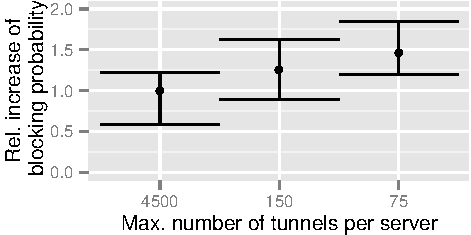
\includegraphics[width=1.0\columnwidth]{figures/blocking-comparison.pdf}
  \caption{Relative increase of blocking probability compared to the traditional \gls{GGSN}; $4500$ maximum tunnels per server being on a single server, $150$ on $30$, and $75$ on $60$ servers.}
\label{fig:blocking-comparison}
  \end{center}
\end{figure}
Next, we take a look at the blocking probability of the virtual \gls{GGSN} system in \reffig{blocking-comparison} and compare it to the results from the traditional \gls{GGSN} model dimensioned for $4500$ concurrent tunnels. We observe that
%, with the start up and shut down time of $5$ minutes in mind, 
the blocking probability increases by a factor of $1.48$ --- albeit at a still very low absolute scale ---  if the capacity of each server is set to $75$, i.e. \nicefrac{1}{60} of the original server capacity, while $27$ of all $60$ servers can be turned of or used for other purposes at $50\%$ of the time. We conclude, that choosing more powerful servers decreases the blocking probability but reduces the potential to disable servers.

\subsection{Impact of startup and shutdown times}
\label{sec:real_virtual_ggsn}
%So far we have considered a conservative start up and shut down time of servers of 5 minutes, which can potentially occur if current generation physical servers are used.
In this section, we first consider the impact of different boot and shut down times, for example if fast flash storage is used, on resource utilization and blocking probabilities. Afterwards, the influence of varying server start and stop times on a fixed combination of maximum tunnels and servers in the system is examined.
\begin{figure*}[htb]
  \begin{center}
  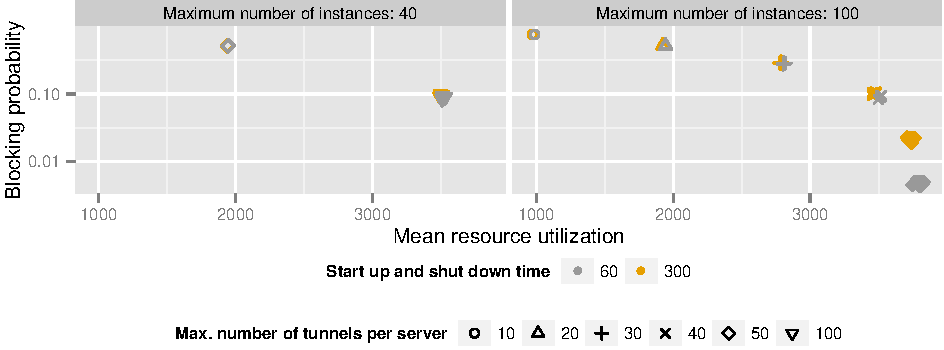
\includegraphics[width=1.0\textwidth]{figures/compare-util-block.pdf}
  \caption{Trade-off between blocking probability and mean resource utilization with regard to maximum number of servers, maximum number of tunnels per server, and start up and shut down time.}
 \label{fig:compare_util_block}
  \end{center}
\end{figure*}
\reffig{compare_util_block} shows scenarios with $40$ and $100$ number of virtual \gls{GGSN} instances surmounting to a total tunnel capacity between $1000$ to $5000$.
We study the impact of selecting different tunnel capacities per virtual instance as well as start up and shut down times on the blocking probability and mean resource utilization.
We observe that by increasing the number of servers, i.e., scaling out, the blocking probability can be decreased, while maintaining a relatively low mean resource utilization.
In addition to the previous effects, we notice that a higher start up and shut down time causes a slight increase in blocking probability for servers with low tunnel capacity.
\begin{figure}[htbp]
  \begin{center}
  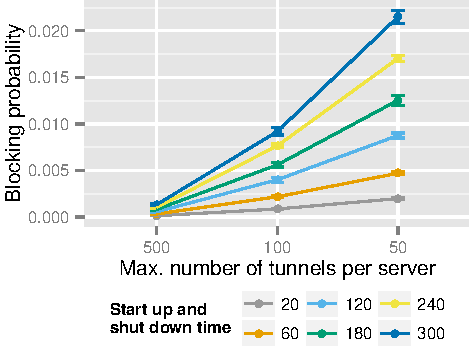
\includegraphics[width=1.0\columnwidth]{figures/compare-maxinstances-block.pdf}
  \caption{Influence of start up and shut down time on blocking probability with regard to different numbers of servers.}
  \label{fig:compare_maxinstances_block}
  \end{center}
\end{figure}
To study this behavior in more detail, we focus on a specific scenario in \reffig{compare_maxinstances_block}, where $5000$ total tunnels should be supported by the system.
In order to achieve this goal, we consider three types of instances, with the server capacity varying between $50$ and $500$. In each case we change the start up and shut down time between $1$ and $5$ minutes.
Lower server capacities combined with higher start up and shut down times increase the blocking probability. This is can in part be attributed to the simplistic instance start up threshold mechanism used in the model, which does not take the additional capacity gained by activating an additional server into account. 
%If a low capacity server with a long boot time is activated, there is a high probability that the system will quickly exhaust its capacity again.
If smaller instances are to be used, for example because they are cheaper than large instances, start up delay should be kept minimal or an appropriate instance management strategy has to be chosen.


%!TEX root = paper.tex
\section{Conclusion}
\label{sec:conclusion}
In this paper we investigated models and trade-offs for virtualizing components of the mobile core network.
We first discussed a novel approach to mobile core network load modeling based on the control plane load at the \gls{GGSN}. The non-stationary Erlang loss model $M(t)/G/c_c/0$ is based on the currently implemented state of the network architecture and backed by an evaluation of actual data. This can serve as a baseline reference to plan and dimension mobile network accordingly, not just based on expected user traffic as traditionally.
To improve scaling in the future, we proposed a new and virtualizable approach for \glspl{GGSN}.
We presented random variables to model load in a \gls{GGSN} based on measurement data from the network of a nation-wide mobile service provider and made them available for reuse.
Finally, we evaluate the model using a queuing simulation. We have shown, that the system's blocking probability is roughly equal to the single-server model but in addition achieves large efficiency gains, even when subjected to rudimentary provisioning conditions and long boot times.
The model also has the ability to very easily scale out one's infrastructure by simply adding more small servers, reducing operational overhead.
Implementing this model in an actual network might need considerable future effort and adaptation of existing infrastructure, protocols and standards. But if done correctly it could lead to new GGSN-as-a-Service business models, removing the need to provide and operate large amounts of infrastructure for rare cases of peak load. 

%In the future we would like to deepen our modeling efforts to provide more dimensioning options for a core network.
% Also, we want to further investigate the correlation of user traffic and signaling and take a look at the implications specific traffic types bring for the core network. 


\printbibliography 

\end{document}
